\section{A Practical Guide to Cloud Optimizer}
\label{sec:guide}

%\subsection{Selecting the Right Optimizer}

\begin{figure*}[t]
 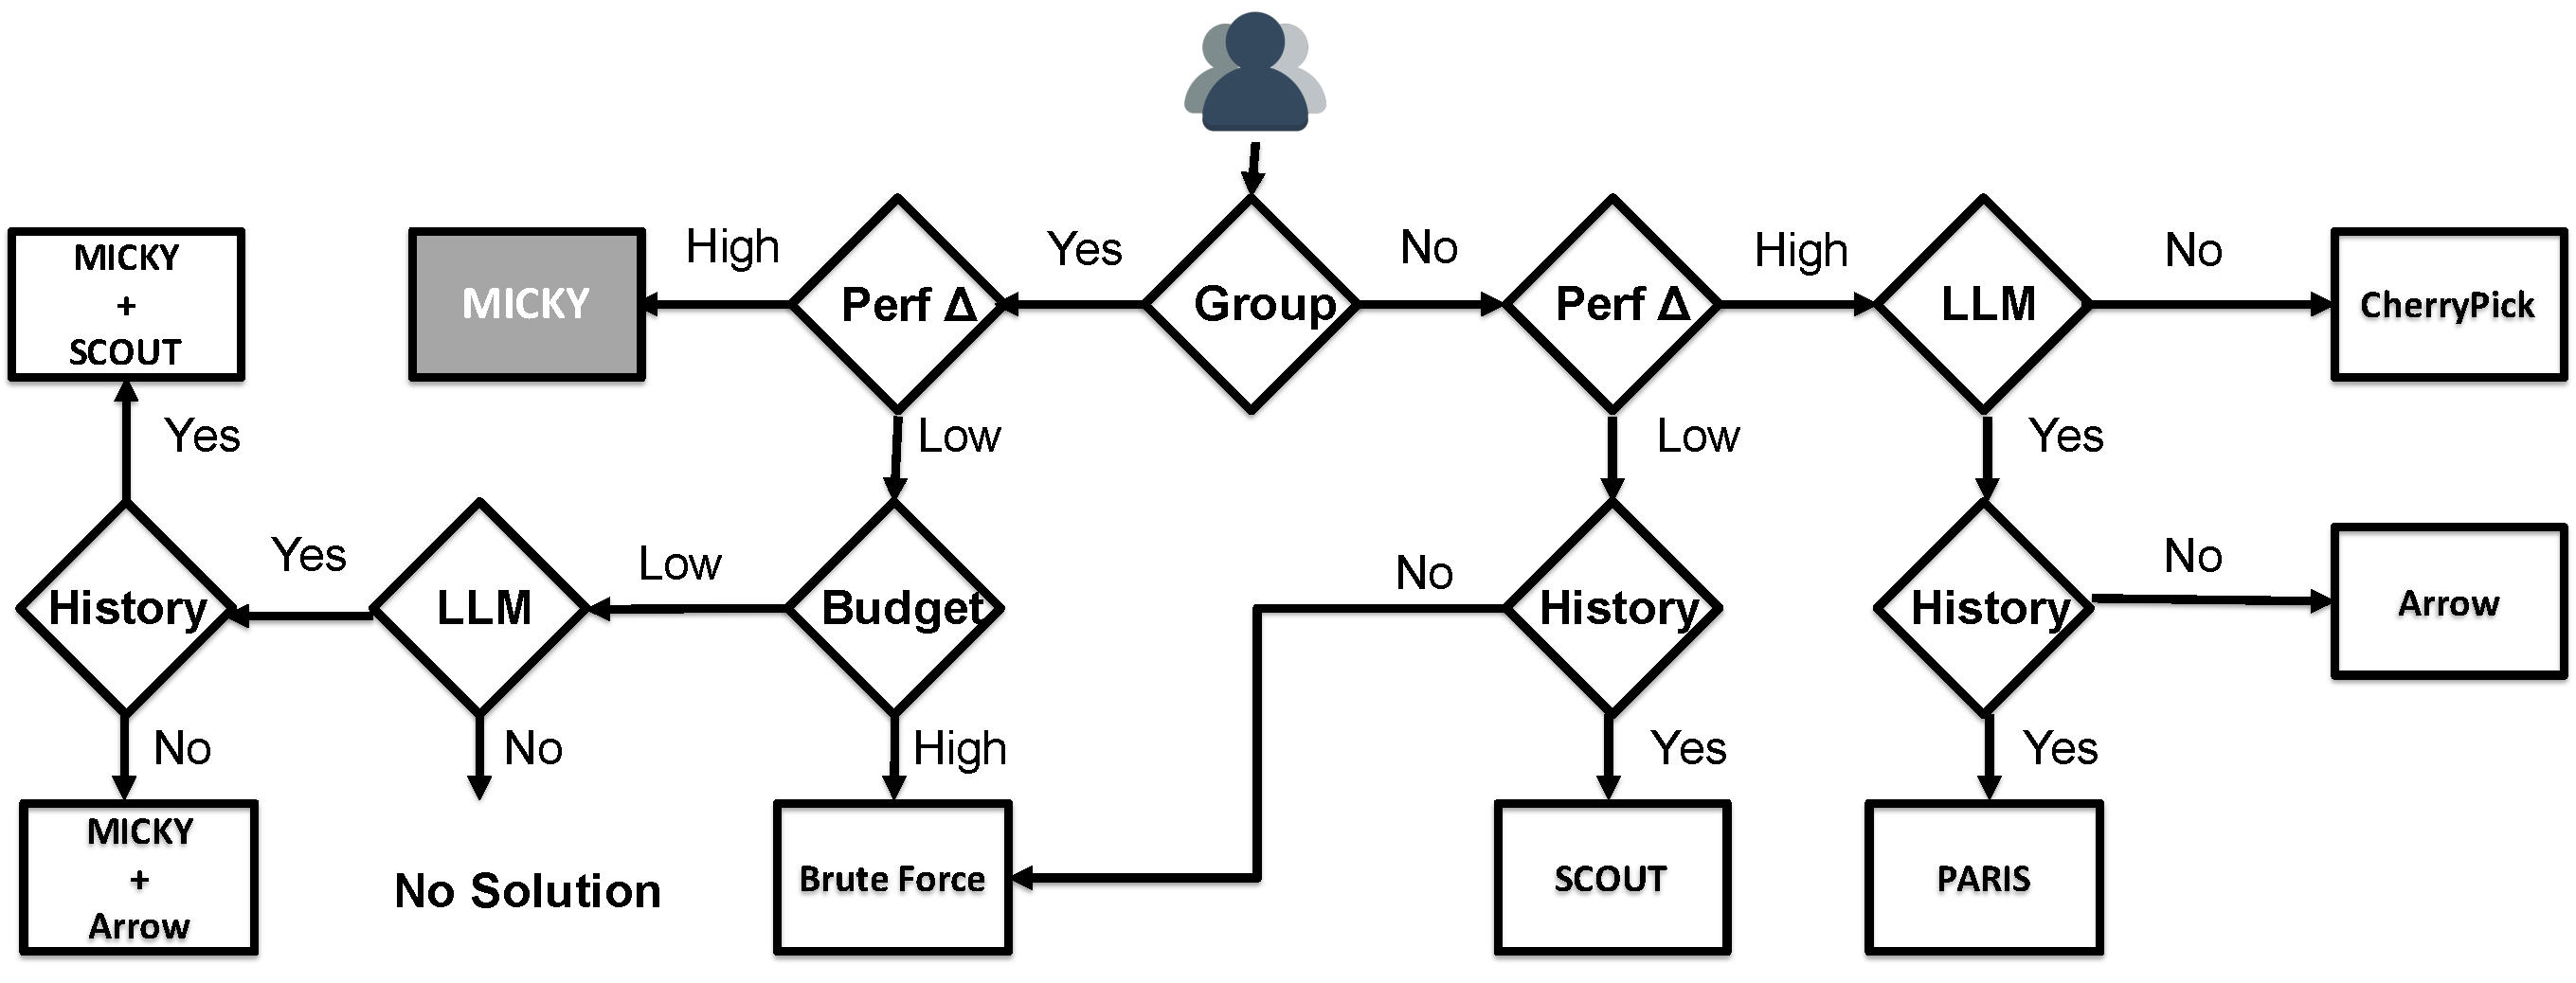
\includegraphics[width=.75\textwidth]{Figures/practical_guide.pdf}
 \vspace*{-2mm}
 \centering
 \caption{\textbf{A practical guide to choosing the right optimization method.} \emph{CheeryPick} works for any workloads without historical and low-level performance data~\cite{Alipourfard2017}. \emph{Arrow} uses low-level metrics to augment Bayesian Optimization (used in \emph{CherryPick})~\cite{Hsu2018Arrow}.  \emph{PARIS} requires low-level and historical data for predicting execution time and running cost of workloads on different VM types~\cite{Yadwadkar2017}.  \scout leverages a learning model and sequential model-based optimization (SMBO) to deliver efficient, effective and reliable recommendation~\cite{Hsu2018Scout}.  \emph{Micky}, different from others, applies collective optimization to largely reduce measurement cost.}
 \label{fig:practical_guide}
 \vspace*{-4mm}
\end{figure*}


To pick an optimizer, we should compare its search performance and measurement cost, and understand their assumptions and constraints.
In \myfigure{\ref{fig:practical_guide}}, we derive a practical guide
for selecting an optimizer.
This guide is derived based on extended literature review and our extensive experimentation.

\textbf{Performance delta (Perf $\Delta$)}
represents search performance, the lower, the better.
Some cloud optimizers may suffer from
the fragility issue or high prediction error.
They are considered less reliable.
When using these optimizers, users should be more careful
because they do not know whether the recommended configurations by the optimizers are near-optimal or sub-optimal.

\textbf{Low-level Metrics (LLM)} are runtime information (such as CPU utilization, memory usage, and I/O rates) for better characterizing
workloads.
If such low-level information is accessible, users should choose optimizers that leverage low-level performance information.

\textbf{Historical data (History)} is execution records of workloads on cloud configurations.
\emph{CherryPick} and \emph{Arrow} do not use historical data (from other workloads) and therefore, require significant initial measurements for 
building prediction models while
\emph{PARIS} and \emph{Scout} uses historical data.

\textbf{Budget} is the measurement cost a user is willing to pay for an optimizer.
While the brute force approach delivers the best search performance,
it is too expensive in practice.
Using the state-of-the-art methods, for example,
\emph{CherryPick} incurs measurement cost of about 22\% to 33\% of the configuration space, and
\emph{Scout} reduces the cost down to 11\% to 19\% while achieving similar or better search performance~\cite{Hsu2018Scout}.

\myfigure{\ref{fig:practical_guide}} summarizes the contribution of this paper.
\micky reduces measurement cost while delivering comparable search performance for a group of workloads.
To address the sub-optimal choices in some workloads, we propose an integration with \scout for further optimization.